\newcommand{\casaapagada}{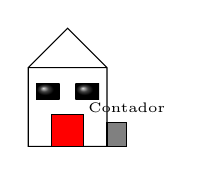
\begin{tikzpicture}
\draw (0,0)--(0,1)--(1/2,3/2)--(1,1)--(1,0)--(0,0)--(0,1)--(1,1);
\shade[shading=ball, ball color=black](0.1,0.6) rectangle (0.4,0.8);
\shade[shading=ball, ball color=black](0.6,0.6) rectangle (0.9,0.8);
\draw[fill=red](0.3,0) rectangle (0.7,0.4);
\draw[fill=gray](1,0) rectangle (1.25,0.3) node[above] {\tiny{Contador}};
\end{tikzpicture}}
\newcommand{\casailuminada}{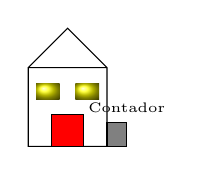
\begin{tikzpicture}
\draw (0,0)--(0,1)--(1/2,3/2)--(1,1)--(1,0)--(0,0)--(0,1)--(1,1);
\shade[shading=ball, ball color=yellow](0.1,0.6) rectangle (0.4,0.8);
\shade[shading=ball, ball color=yellow](0.6,0.6) rectangle (0.9,0.8);
\draw[fill=red](0.3,0) rectangle (0.7,0.4);
\draw[fill=gray](1,0) rectangle (1.25,0.3) node[above] {\tiny{Contador}};
\end{tikzpicture}}

\newcommand{\hombrecito}{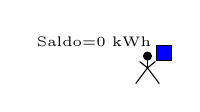
\begin{tikzpicture}
\draw (0,0)--(0.15,0.2)--(0.3,0);
\draw (0.15,0.2)--(0.05,0.28);
\draw (0.15,0.2)--(0.25,0.28);
\draw (0.15,0.2)--(0.15,0.3);
\draw[fill=black] (0.15, 0.35) circle (.05);
\draw[fill=blue] (0.26,0.29) rectangle (0.45,0.48) node[pos=0.3,above left] {\tiny{Saldo=0 kWh}};
\end{tikzpicture}}

\newcommand{\hombrecitoo}{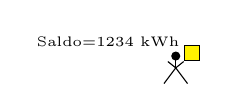
\begin{tikzpicture}
\draw (0,0)--(0.15,0.2)--(0.3,0);
\draw (0.15,0.2)--(0.05,0.28);
\draw (0.15,0.2)--(0.25,0.28);
\draw (0.15,0.2)--(0.15,0.3);
\draw[fill=black] (0.15, 0.35) circle (.05);
\draw[fill=yellow] (0.26,0.29) rectangle (0.45,0.48) node[pos=0.3,above left] {\tiny{Saldo=1234 kWh}};
\end{tikzpicture}}

\newcommand{\familiafeliz}{
\begin{tikzpicture}
\draw (0,0)--(0.15,0.2)--(0.3,0);
\draw (0.15,0.2)--(0.05,0.28);
\draw (0.15,0.2)--(0.25,0.28);
\draw (0.15,0.2)--(0.15,0.3);
\draw[fill=black] (0.15, 0.35) circle (.05);
\end{tikzpicture}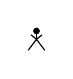
\begin{tikzpicture}[scale=0.7]
\draw (0,0)--(0.15,0.2)--(0.3,0);
\draw (0.15,0.2)--(0.05,0.28);
\draw (0.15,0.2)--(0.25,0.28);
\draw (0.15,0.2)--(0.15,0.3);
\draw[fill=black] (0.15, 0.35) circle (.05);
\end{tikzpicture}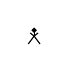
\begin{tikzpicture}[scale=0.5]
\draw (0,0)--(0.15,0.2)--(0.3,0);
\draw (0.15,0.2)--(0.05,0.28);
\draw (0.15,0.2)--(0.25,0.28);
\draw (0.15,0.2)--(0.15,0.3);
\draw[fill=black] (0.15, 0.35) circle (.05);
\end{tikzpicture}\begin{tikzpicture}[scale=0.2]
\draw (0,0)--(0.15,0.2)--(0.3,0);
\draw (0.15,0.2)--(0.05,0.28);
\draw (0.15,0.2)--(0.25,0.28);
\draw (0.15,0.2)--(0.15,0.3);
\draw[fill=black] (0.15, 0.35) circle (.05);
\end{tikzpicture}}


\section{Introducción}

%\begin{wrapfigure}{r}{0.5\textwidth} 
%\vspace{-1cm}
%  \begin{figurebox}
%    \vspace{0.1cm}
%  \centering
%  \includegraphics[width=\textwidth]{TuberiaMolecor.jpg}
%  \caption{Tuberías  TOM\textcopyright \,  PVC-0 de Molecor.}
%  \label{fig:1}
%\end{figurebox}
%\end{wrapfigure}

 Un {\sl sistema de prepago} consiste en la anticipación del importe del consumo que se realizará. Este consumo puede ser de diferentes servicios: servicio telefónico, servicio de transporte público o servicios de agua y luz entre otros. En este artículo nos vamos a focalizar en explicar con detenimiento que es un sistema de prepago eléctrico que se ha puesto tan popular en los últimos años en Ángola.

 Un {\sl sistema de prepago eléctrico} consiste en que el cliente debe pagar con anticipación la cantidad que consumirá, recargando por ejemplo una tarjeta por cierto valor monetario asignados al kilovatio-hora (\kilowatthour) que son ingresadas a un medidor de electricidad electrónico instalado en el hogar o en un recinto específico. Así, la cantidad de energía que circulará hacia la casa estará restringida al total del valor ingresado en el medidor. 

El origen de los sistemas prepagos está basado en los contadores mecánicos que se desarrollaron en Estados Unidos a principio del siglo pasado y que funcionaban con monedas. El sistema de prepago de energía partió en Sudáfrica en 1988. Desde ahí se ha expandido hacia otros continentes.

Este sistema permite regular el consumo y el gasto, ya que el cliente sólo tendrá que pagar por los vatios que haya gastado en su estancia. De este modo la economía de una familia está más controlada por ellos mismos y se evita fraude y morosidad en los pagos.

\section{Elementos de un sistema de prepago}

\begin{figure}[ht!]
\begin{figurebox}
    \begin{subfigure}{.2\textwidth}
  \centering
   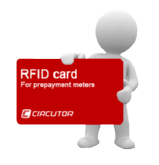
\includegraphics[height=50pt]{tarjeta.png}
   \caption{Tarjeta prepago}
\end{subfigure}
 \begin{subfigure}{.2\textwidth}
  \centering
   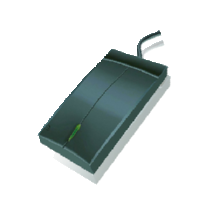
\includegraphics[height=50pt]{control.png}
   \caption{Control tarjeta}
\end{subfigure}
\begin{subfigure}{.2\textwidth}
\centering
  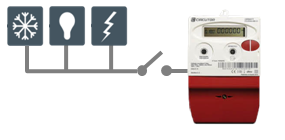
\includegraphics[height=50pt]{ContadorMonofasico.png}
  \caption{Contador}
 \end{subfigure}
 \begin{subfigure}{.2\textwidth}
  \centering
   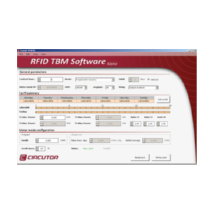
\includegraphics[height=50pt]{software.png}
   \caption{Tarjeta prepago}
\end{subfigure} \caption{Ejemplo de elementos de un sistema de prepago:\\ Sistema de prepago de Circutor.} \label{figure:elementos}
\end{figurebox}
\end{figure}

Existen diferentes alternativas de sistemas de prepago: dinero electrónico, sistema de puntos y descuentos, cuentas virtuales y sistema eMetal. Nosotros vamos a focalizarnos en el primer tipo, esto es dinero electrónico y en particular vamos a hablar a través de tarjetas de prepago con tecnología RFID. Los principales elementos de un sistema prepago eléctrico vanguardista como el que mencionamos aquí son los siguientes(véase Figura \ref{figure:elementos}):
\begin{enumerate}
\item Tarjeta RFID: es una tarjeta plástica (en general de PVC) que tiene implementado el sistema RFID, esto es {\bf R}adio {\bf F}requency {\bf ID}entification, en español identificación por radiofrecuencia; es un sistema de almacenamiento y recuperación de datos remoto. El propósito fundamental de la tecnología RFID es transmitir la identidad de un objeto mediante ondas de radio.
\item Control de la tarjeta RFID: es el equipo encargado de leer y grabar las tarjetas RFID.
\item Los contadores tanto monofásicos como trifásicos.
\item Software: que permite la gestión de ls elementos anteriores.
\end{enumerate}


En norma general, tanto el control de la tarjeta como el software estará a disposición de ciertos lugares físicos que controlarán la carga de las tarjetas. Sobre todo este funcionamiento tiene sentido en lugares donde el acceso a internet es limitado. en caso contrario, la carga y la administración de la tarjeta se podría hacer mediante internet desde portales que la empresa distribuidora que oferta el servicio posee a disposición del cliente.

\section{Ventajas de un sistema de prepago}
Un sistema de prepago tiene ventajas tanto para el usuario como para la distribuidora eléctrica. Respecto al usuario las ventajas pueden ser resumidas como sigue:
\begin{dinglist}{52}
\item Mejora la administración del presupuesto familiar.
\item Es un sistema fácil de usar.
\item No hay facturas a final de mes.
\item No hay errores humanos en las lecturas de los contadores energéticos.
\item Proporciona información de la energía consumida, dando al usuario un conocimiento real de como economizar sus gastos energéticos.
\end{dinglist}
Respecto a la distribuidora eléctrica, las ventajas son las siguientes:
\begin{dinglist}{76}
\item Facilita el cobro de la energía.
\item Reduce los costos de operación y de lectura.
\item Mejora el control del fraude y el control de cargas.
\end{dinglist}

\section{Funcionamiento}

Vamos a hacer una simple representación del funcionamiento del sistema de prepago para el gasto energético presuponiendo que lo haremos mediante una tarjeta prepago y que existe físicamente en su localidad un distribuidor que permite el cargo de la tarjeta. Para optar a este servico, usted debe tener implementado en su hogar el contador monofásico o trifásico según corresponda a sus instalaciones eléctricas. Deberá ir al distribuidor con su tarjeta RFID para que se produzca el cargo de dicha tarjeta a cambio de dinero. Una vez cargada la tarjeta debe llevarla a su contador en su domicilio y pasarle la información (esto se hace mediante las radiofrecuencias antes mencionadas). De este modo ya puede hacer uso eléctrico en su hogar hasta que el saldo de su tarjeta quede vacío. No olvide leer los consejos que le damos para tener un ahorro energético en su hogar (veáse Sección \ref{ahorro}). 

Puede ir controlando el saldo que le va quedando tantas veces como usted quiera acercando su tarjeta al contador y así poder gestionar que aparatos son los más costosos y gestionar su ahorro. Cuando el saldo se le acaba o está a punto de agotarse, volvemos al punto de inicio, cargar la tarjeta en su distribuidor o mediante internet. Una divertida ilustración puede ser vista en la Fígura \ref{fig2} sobre el funcionamiento de este sistema prepago.

\begin{figure}[ht!]
\begin{figurebox} 
\begin{center}
\casaapagada \tikz \draw[-] (0,0) -- (2,0) node[pos=0.5,above]{\hombrecito};
\tikz \draw[fill=green](3.1,3.1) rectangle (4.1,4.1) node[above left]{\tiny{Distribuidor}};
\tikz \draw[-] (0,0) -- (2,0) node[pos=0.5,above]{\hombrecitoo};
\casaapagada \hombrecitoo
\tikz \draw[->] (0,0) -- (2,0);
\casailuminada \familiafeliz
\end{center}\caption{Animación del proceso de tarjeta prepago.}\label{fig2}
\end{figurebox}
\end{figure}


\section{Sistema multimodo: sus opciones}
Este tipo de tarjetas prepago RFID pueden ser más operativas que lo mencionado hasta ahora permitiendo diferentes modalidades de uso de estas. Por ejemplo, podemos hablar de unas tarjetas RFID multipago que son creadas por la empresa Circutor (\url{www.circutor.com}). Estas poseen varios modos de uso. Aquí le explicamos alguno de ellos para que se haga a la idea de las múltiples opciones que puede encontrar con un sistema prepago.
\begin{dinglist}{224}
\item \textsl{Modo prepago sin recuperación de energía:} el saldo en \kilowatthour \: es introducido mediante una tarjeta y cuando se agota el crédito, el contador abre el elemento de corte integrado en el propio equipo y no se cierra hasta que el usuario ha cargado la tarjeta RFID con saldo positivo.
\item \textsl{Modo prepago con recuperación de energía:} este modo funciona similar al anterior con el añadido que si el contador posee saldo positivo este puede ser transpasado nuevamente a la tarjeta RFID y esta ser usada en otros contadores. 
\item \textsl{Modo de crédito:} existe un contrato con fecha de caducidad expresado en días desde la última recarga, en ese tiempo el usuario consume libremente energía. Periodicamente el usuario debe pasar la tarjeta hasta la fecha. Una vez satisfecho el pago de este consumo en la tarjeta se grabará los días de validez hasta la nueva facturación.
\item \textsl{Modo dispensador básico:} el cliente contrará un consumo en \kilowatthour \: máximo al día. El totalizador de energía se recarga cada segundo con la energía resultante de dividir la energía contratada a $86.400$ segundos que posee un día. Si el consumo de energía es superior a la carga que se realice en función de la potencia contratada, el contador corta el suministro. Y, en el caso opuesto, que no exista consumo, el crédito se irá llenando hasta alcanzar como máximo el equivalente a un número fijo de días, digamos tres. En la configuración del contador de prepago se define un umbral que consiste un porcentaje del consumo máximo permitido por día según la potencia contratada. Si estando el elemento de corte abierto supera este umbral de carga entonces el contador recupera el suministro.
\end{dinglist}

\section{Seguridad en un sistema prepago}


Cuando se recarga la tarjeta que se usa para el sistema prepago la información en ella queda encriptada y cuando se acerca al contador este es el encargado de desenpcritarla y convertirla en energía disponible por el usuario. El proceso de encriptación y desencriptación se hace mediante el algoritmo AES, Advanced Encryptation Standard que es el algoritmo del que hemos hablado en la sección de Matemática en INgeniería. No te lo pierdas. 

Como curiosidad, contarles que un grupo de investigadores de Microsoft y de la Dutch Katholieke Universiteit Leuven han descubierto una manera de romper este sistema AES. Los investigadores nos dejan algo más tranquilos cuando aseguran que romper esta seguridad es algo complejo y costoso: serían necesarios un billón de ordenadores que pudieran cada uno probar mil millones de claves por segundo y tardarían más de 2.000 millones de años en dar con una del sistema AES-128. 

\section{Consejos para ahorro de energía en su hogar}\label{ahorro}
%\begin{wrapfigure}{r}{0.5\textwidth}\vspace{-1cm}
%  \begin{figurebox}%\vspace{0.25cm}
%    \centering 
%  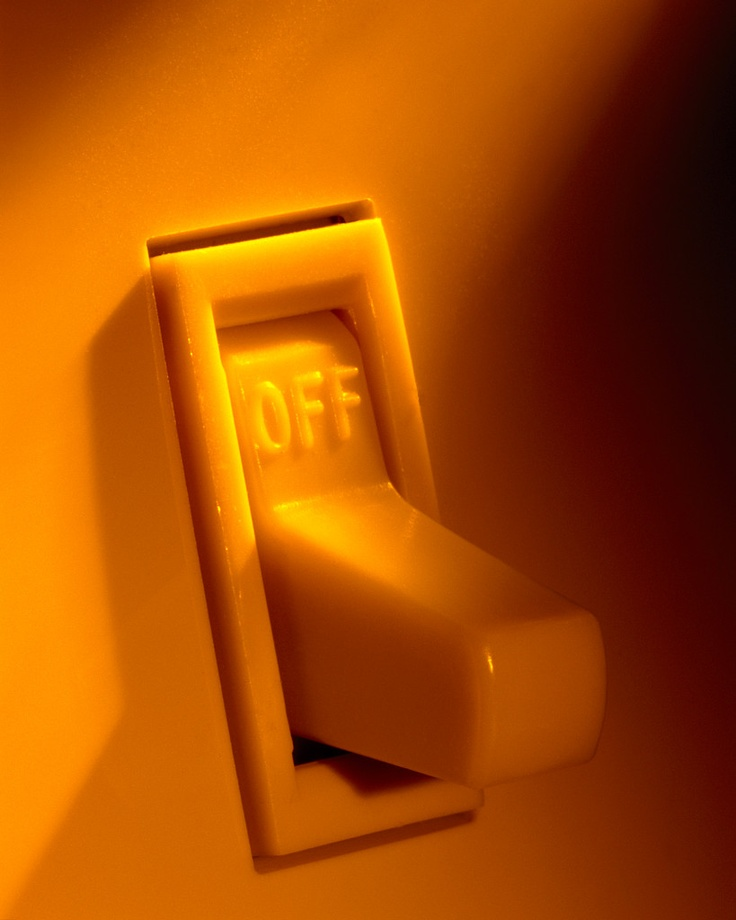
\includegraphics[scale=0.05]{ahorro.jpg}
%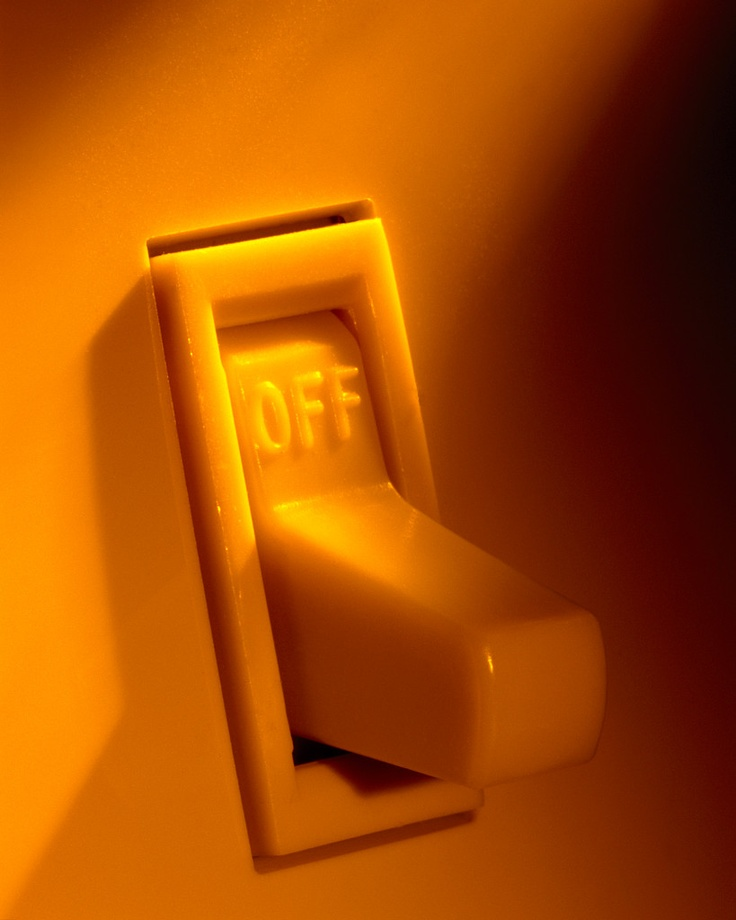
\includegraphics[scale=0.05]{ahorro.jpg}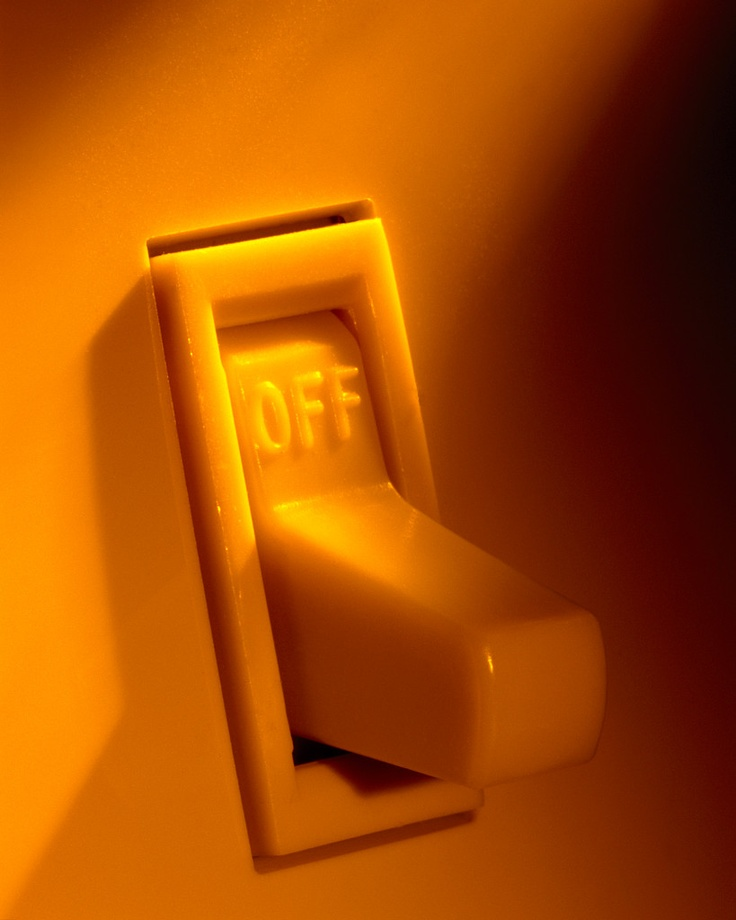
\includegraphics[scale=0.05]{ahorro.jpg}
%  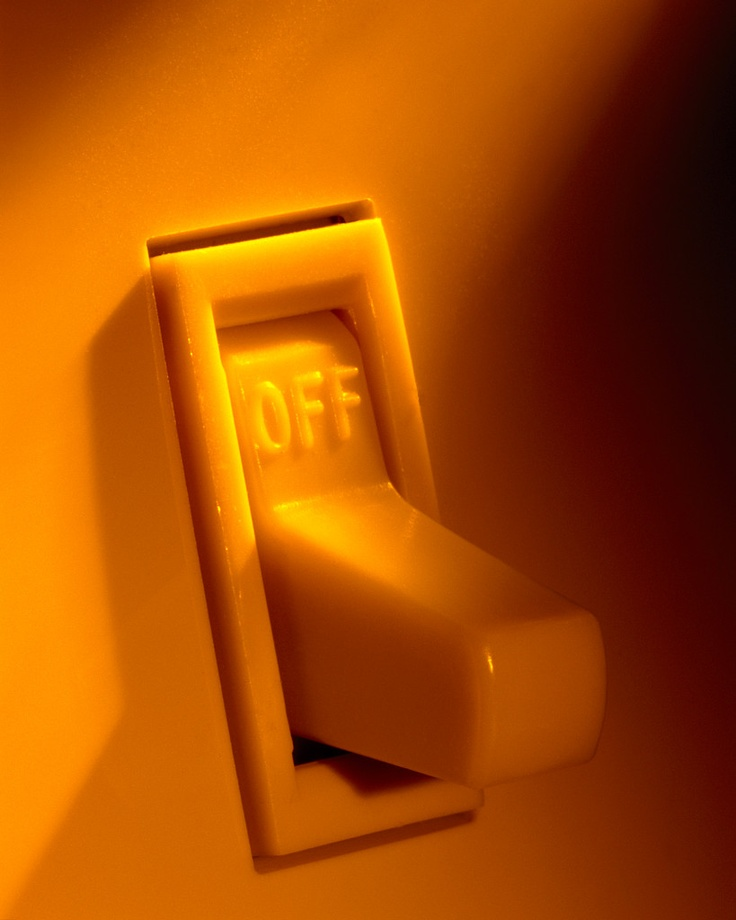
\includegraphics[scale=0.05]{ahorro.jpg}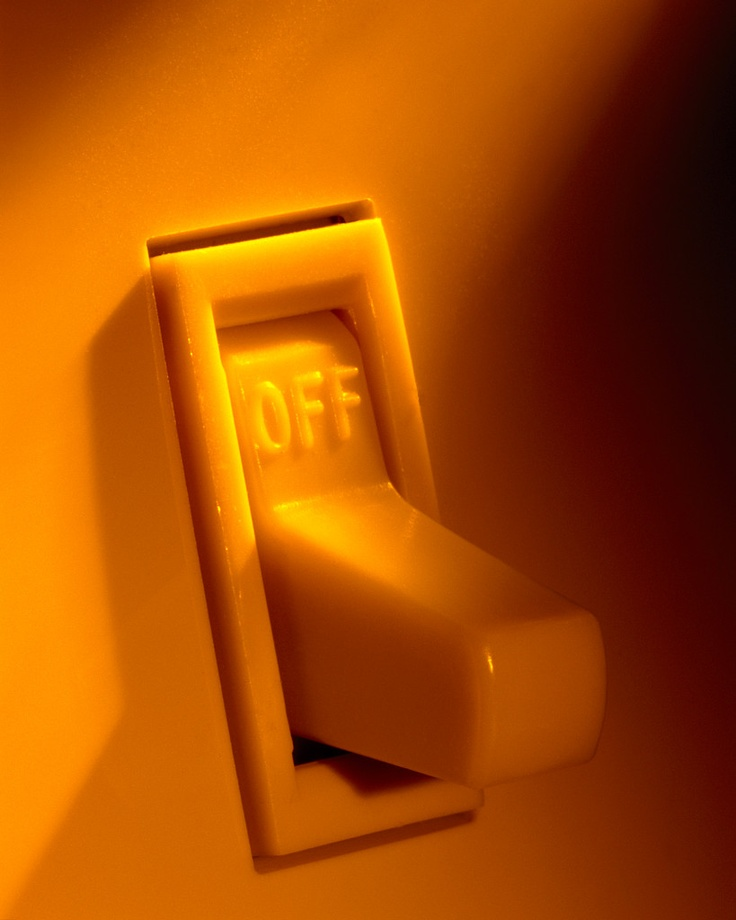
\includegraphics[scale=0.05]{ahorro.jpg}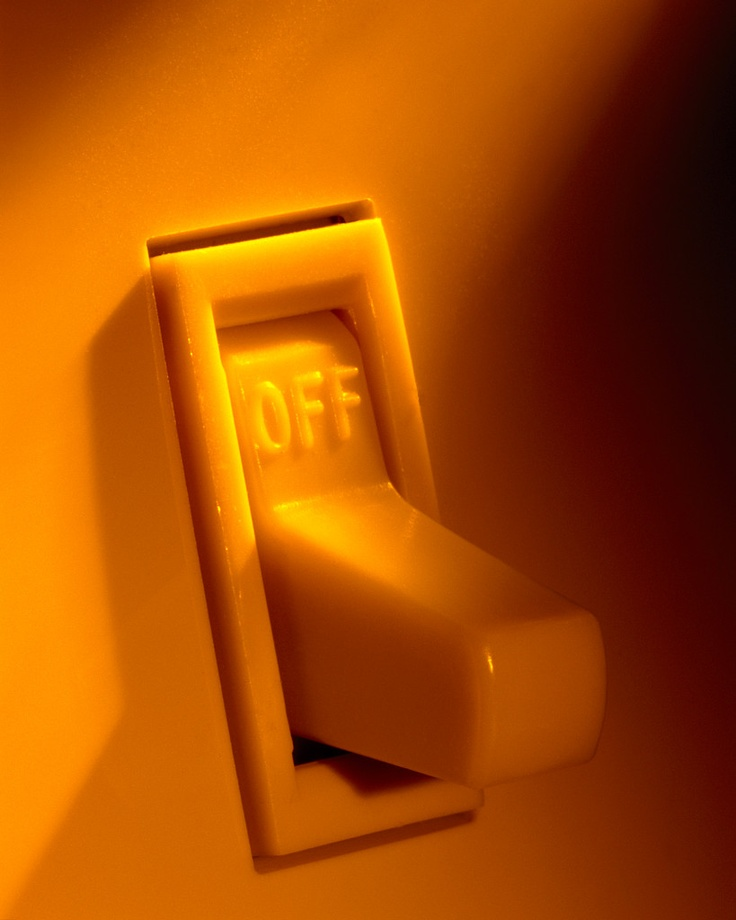
\includegraphics[scale=0.05]{ahorro.jpg}
%\end{figurebox}\vspace{-0.25cm}
%\end{wrapfigure}
Estos son algunos consejos para el ahorro de energía en su hogar. 
  \begin{dinglist}{100}
  \item Descongelar periódicamente su refrigerador le permitirá ahorrar energía y dinero. 
  \item Abra el refrigerador sólo cuando sea necesario y por la menor cantidad de tiempo posible, así evitará la pérdida de frío. 
  %\item Mantenga el congelador lo más lleno posible, los alimentos congelados ayudan a conservar el frío. Si es necesario, llene con agua algunos recipientes, tápelos e introdúzcalos en el congelador. 
  \item No introduzca alimentos calientes en el refrigerador. 
  \item Aproveche al máximo la luz natural. Además, evite encender luces durante el día y apague las luces que no está usando. 
  \item Cambie sus bombillas tradicionales (incandescentes) por las de ahorro de energía. Empiece por aquellas que más tiempo tiene encendida.
 % \item Pinte su casa con colores claros. Los colores oscuros requieren más iluminación.
 \item Limpie regularmente bombillas y lámparas para tener la iluminación adecuada.

% \item Lave a carga completa y con agua fría. 
% \item Planche una sola vez para evitar la desconexión constante de la plancha.  
% \item Si va a utilizar lavadoras, secadoras de ropa o lavavajillas automáticas utilice carga completa y siempre limpie los filtros de los artefactos que use, una vez que termine su uso, sobre todo en el caso de las aspiradoras y secadoras.
% \end{dinglist}
%\item Cocina:
%\begin{dinglist}{167}
%\item Las ollas o recipientes deben ser del tamaño de la hornilla. Si utiliza recipientes con una superficie mayor al calentador, se alarga el período de cocción. %
%\item Utilice al máximo la olla de presión para cocinar.
%\item Use termos para mantener calientes sus bebidas.  Si usted toma café varias veces al día, hágalo sólo en la mañana y guárdelo inmediatamente en un termo. 
%\end{dinglist}
%\item Equipos Electrónicos:
% \begin{dinglist}{37}
 %\item  Entre un 15\% y 20\% de ahorro de energía se puede lograr apagando y desenchufando los equipos electrónicos que no utilice regularmente (DVD, Video, Consolas de Juego). 
 %\item Configure su computador en “función de ahorro” y apague la pantalla si va a salir por más de media hora.
%\end{dinglist}
\end{dinglist}

%\newpage
\noindent
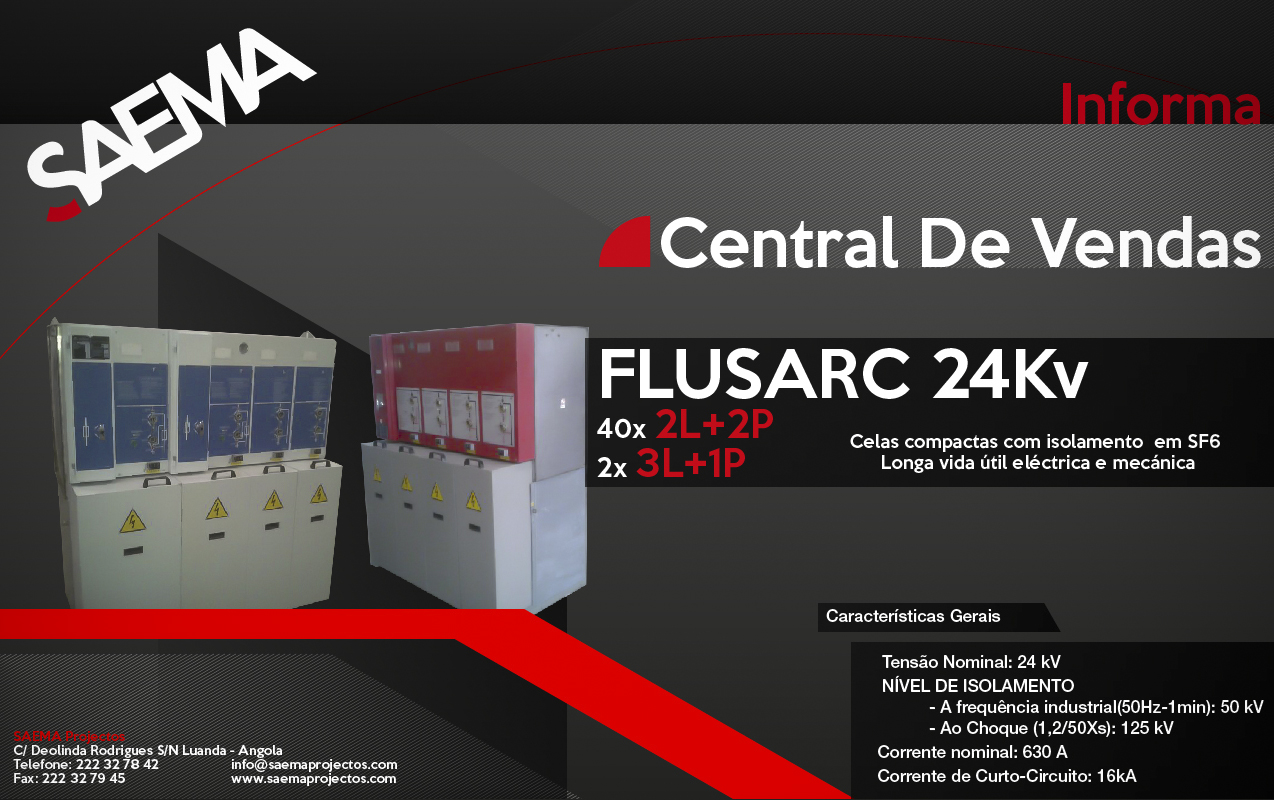
\includegraphics[width=\textwidth,scale=0.3]{aihbbgje.jpg}


\newpage
%%% Local Variables: 
%%% mode: latex
%%% TeX-master: "novedades"
%%% End: 


